% This is a Basic Assignment Paper but with like Code and stuff allowed in it, there is also url, hyperlinks from contents included. 

\documentclass[11pt]{article}

% Preamble

\usepackage[margin=1in]{geometry}
\usepackage{amsfonts, amsmath, amssymb}
\usepackage{fancyhdr, float, graphicx}
\usepackage[utf8]{inputenc} % Required for inputting international characters
\usepackage[T1]{fontenc} % Output font encoding for international characters
\usepackage{fouriernc} % Use the New Century Schoolbook font
\usepackage[nottoc, notlot, notlof]{tocbibind}
\usepackage{listings}
\usepackage{xcolor}
\usepackage{blindtext}
\usepackage{hyperref}
\usepackage{booktabs}
\hypersetup{
    colorlinks=true,
    linkcolor=black,
    filecolor=magenta,      
    urlcolor=cyan,
    pdfpagemode=FullScreen,
    }

\definecolor{codegreen}{rgb}{0,0.6,0}
\definecolor{codegray}{rgb}{0.5,0.5,0.5}
\definecolor{codepurple}{rgb}{0.58,0,0.82}
\definecolor{backcolour}{rgb}{0.95,0.95,0.92}

\lstdefinestyle{mystyle}{
    backgroundcolor=\color{backcolour},   
    commentstyle=\color{codegreen},
    keywordstyle=\color{magenta},
    numberstyle=\tiny\color{codegray},
    stringstyle=\color{codepurple},
    basicstyle=\ttfamily\footnotesize,
    breakatwhitespace=false,         
    breaklines=true,                 
    captionpos=b,                    
    keepspaces=true,                 
    numbers=left,                    
    numbersep=5pt,                  
    showspaces=false,                
    showstringspaces=false,
    showtabs=false,                  
    tabsize=2
}

\lstset{style=mystyle}

% Header and Footer
\pagestyle{fancy}
\fancyhead{}
\fancyfoot{}
\fancyhead[L]{\textit{\Large{Advanced Data Structures - Assignment 9}}}
%\fancyhead[R]{\textit{something}}
\fancyfoot[C]{\thepage}
\renewcommand{\footrulewidth}{1pt}



% Other Doc Editing
% \parindent 0ex
%\renewcommand{\baselinestretch}{1.5}

\begin{document}

\begin{titlepage}
    \centering

    %---------------------------NAMES-------------------------------

    \huge\textsc{
        MIT World Peace University
    }\\

    \vspace{0.75\baselineskip} % space after Uni Name

    \LARGE{
        Advanced Data Structures\\
        Second Year B. Tech, Semester 4
    }

    \vfill % space after Sub Name

    %--------------------------TITLE-------------------------------

    \rule{\textwidth}{1.6pt}\vspace*{-\baselineskip}\vspace*{2pt}
    \rule{\textwidth}{0.6pt}
    \vspace{0.75\baselineskip} % Whitespace above the title



    \huge{\textsc{
            Implementation of AVL as a Data Structure
        }} \\



    \vspace{0.5\baselineskip} % Whitespace below the title
    \rule{\textwidth}{0.6pt}\vspace*{-\baselineskip}\vspace*{2.8pt}
    \rule{\textwidth}{1.6pt}

    \vspace{1\baselineskip} % Whitespace after the title block

    %--------------------------SUBTITLE --------------------------	

    \LARGE\textsc{
        Assignment No. 9
    } % Subtitle or further description
    \vfill

    %--------------------------AUTHOR-------------------------------

    Prepared By
    \vspace{0.5\baselineskip} % Whitespace before the editors

    \Large{
        Krishnaraj Thadesar \\
        Cyber Security and Forensics\\
        Batch A1, PA 20
    }


    \vspace{0.5\baselineskip} % Whitespace below the editor list
    \today

\end{titlepage}

\tableofcontents
\thispagestyle{empty}
\clearpage

\setcounter{page}{1}

\section{Objectives}
\begin{enumerate}
    \item 1. To study the concept of AVL trees
    \item 2. To study different rotations applied on AVL tree
\end{enumerate}

\section{Problem Statement}
\textit{A Dictionary stores keywords and its meaning. Provide facility for adding new keywords, deleting keywords, updating values of any entry. Provide facility to display whole data sorted in ascending/ Descending order. Also find how many maximum comparisons may require for finding any keyword. Use Height balance tree and find the complexity for finding a keyword.}
\section{Theory}
\begin{quotation}
    An AVL (Adelson-Velskii and Landis) tree is a self-balancing binary search tree in which the heights of the left and right subtrees of any node differ by at most one. The balancing property of AVL trees ensures that the worst-case time complexity of search, insert and delete operations is O(log n), where n is the number of nodes in the tree.\\

    The height of a node is the number of edges in the longest path from the node to a leaf. An AVL tree is balanced if and only if the heights of its left and right subtrees differ by at most one. If the height difference is more than one, the tree is rebalanced by performing one or more rotations.
\end{quotation}

\begin{figure}[H]
    \centering
    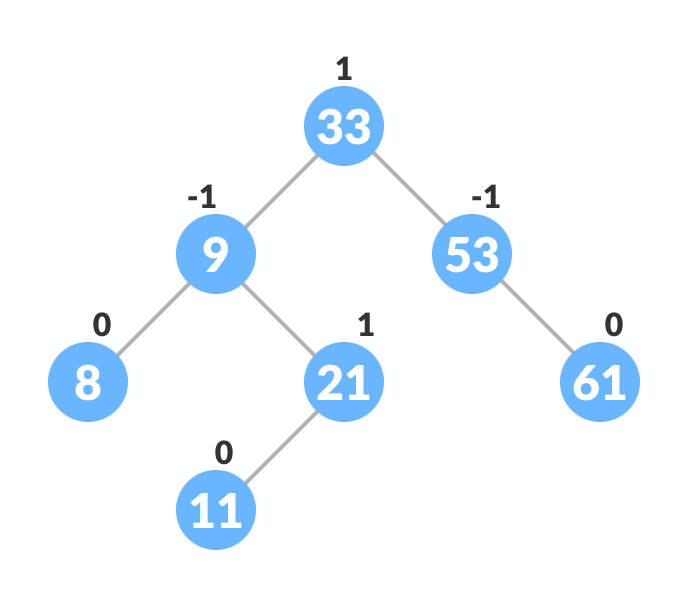
\includegraphics[width=.45\textwidth]{avl-tree-final-tree-1_0_2.png}
    \caption{Example of an AVL Tree}
\end{figure}

\subsection{Different Cases of Rotations in AVL Tree}

There are four possible cases of rotation in AVL trees:
\begin{enumerate}
    \item \textit{Left-Left (LL)}:  Case: This case occurs when the height of the left subtree of a node is greater than the height of the right subtree by more than one, and the height of the left subtree's left child is greater than or equal to the height of its right child. To fix this, we perform a right rotation at the unbalanced node.
    \item \textit{Right-Right (RR)}:  Case: This case occurs when the height of the right subtree of a node is greater than the height of the left subtree by more than one, and the height of the right subtree's right child is greater than or equal to the height of its left child. To fix this, we perform a left rotation at the unbalanced node.
    \item \textit{Left-Right (LR)}:  Case: This case occurs when the height of the left subtree of a node is greater than the height of the right subtree by more than one, and the height of the left subtree's right child is greater than the height of its left child. To fix this, we perform a left rotation at the left child, followed by a right rotation at the unbalanced node.
    \item \textit{Right-Left (RL)}:  Case: This case occurs when the height of the right subtree of a node is greater than the height of the left subtree by more than one, and the height of the right subtree's left child is greater than the height of its right child. To fix this, we perform a right rotation at the right child, followed by a left rotation at the unbalanced node.

\end{enumerate}
\subsection{Construction of AVL Tree as a Data Structure for Creation of Dictionary}

AVL trees are commonly used as data structures for the creation of dictionaries. A dictionary is a collection of key-value pairs, where each key is associated with a value. In an AVL tree-based dictionary, the keys are stored in the tree, and the associated values are stored in the nodes.\\

To construct an AVL tree-based dictionary, we start with an empty AVL tree. For each key-value pair to be inserted, we perform a binary search in the tree to find the correct position for insertion. If the key is already present in the tree, we update its value. If the key is not present, we create a new node with the key-value pair and insert it into the tree. After insertion, we check if the tree is still balanced. If it is not, we perform one or more rotations to balance it.\\

\begin{figure}[H]
    \centering
    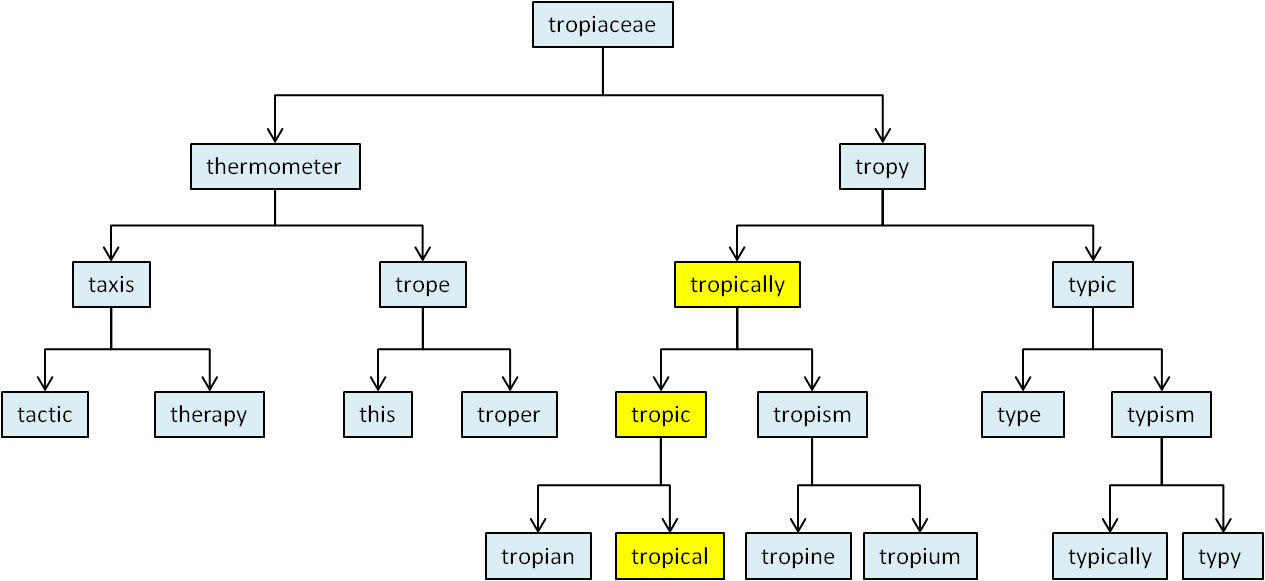
\includegraphics[width=.85\textwidth]{balanced_bst2.png}
    \caption{Example of an AVL Tree being used as a Dictionary}
\end{figure}

\subsection{Searching and Deleting in AVL Tree}

To search for a key in the AVL tree-based dictionary, we perform a binary search in the tree. If the key is found, we return its associated value. Otherwise, we return a null value to indicate that the key is not present in the dictionary.\\

To delete a key from the AVL tree-based dictionary, we perform a binary search to find the node containing the key. If the key is found, we delete the node and perform one or more rotations to balance the tree if necessary. If the node to be deleted has two children, we replace it with the successor or predecessor node, which is the node with the smallest or largest key in its right or left subtree, respectively.

\subsection{Advantages of AVL Tree over Other Data Structures}

The AVL tree-based dictionary has several advantages over other data structures, such as hash tables or binary search trees.

\begin{enumerate}
    \item AVL trees are self-balancing, which means that the height of the left and right subtrees of any node differ by at most one. This ensures that the worst-case time complexity of search, insert, and delete operations is O(log n), where n is the number of nodes in the tree. Hash tables have an average-case time complexity of O(1), but their worst-case time complexity can be O(n) if all the keys hash to the same slot. Binary search trees have a worst-case time complexity of O(n) if the tree is unbalanced.

    \item AVL trees are more space-efficient than hash tables. The space complexity of an AVL tree is O(n), where n is the number of nodes in the tree. The space complexity of a hash table is O(n), where n is the number of key-value pairs in the table.

    \item AVL trees have a guaranteed worst-case time complexity of O(log n) for search, insert, and delete operations, regardless of the distribution of the keys. Hash tables have an average-case time complexity of O(1), but their worst-case time complexity can be O(n) if all the keys hash to the same slot. Binary search trees have a worst-case time complexity of O(n) if the tree is unbalanced.
\end{enumerate}

\subsection{Disadvantages of AVL Tree over Other Data Structures}

\begin{enumerate}
    \item Overhead: Maintaining the balance of AVL trees requires additional operations and memory compared to regular binary search trees, which can add overhead to the implementation.

    \item Rotations: Whenever an insertion or deletion violates the balance condition of an AVL tree, rotations are required to restore the balance. These rotations can be complex and time-consuming, especially in larger trees.

    \item Limited use: AVL trees are not always the best choice for certain types of applications. For example, in situations where insertions and deletions are infrequent and searches are more common, a simple binary search tree may be a better choice.

    \item Implementation complexity: Implementing an AVL tree can be more complex than implementing a regular binary search tree, which can lead to more errors and bugs in the code.

    \item Memory overhead: In some cases, AVL trees may consume more memory than other types of binary search trees, due to their need to maintain balance. This can be a concern in memory-constrained environments or when dealing with very large data sets.
\end{enumerate}


\section{Platform}
\textbf{\textbf{Operating System}}: Arch Linux x86-64 \\
\textbf{\textbf{IDEs or Text Editors Used}}: Visual Studio Code\\
\textbf{\textbf{Compilers} }: g++ and gcc on linux for C++\\

\section{Test Conditions}
\begin{enumerate}
    \item Input min 10 elements.
\end{enumerate}

\section{Input and Output}
\begin{enumerate}
    \item The Elements in Ascending Order, or Descending order
\end{enumerate}

\section{Pseudo Code}
\subsubsection*{Pseudo Code for Creation of AVL Trees}
\begin{lstlisting}[language=C++]
    struct Node
        string word
        string definition
        struct Node *l
        struct Node *r
        friend class AVL_Tree
    
    class AVL_Tree
    public:
        Node *head
        AVL_Tree()
            head = new Node
            head->l = NULL
            head->r = NULL
            head->definition = "AVL Dictionary"
            head->word = "Head"
\end{lstlisting}

\subsubsection*{Pseudo Code for Rotations of AVL Trees}
\begin{lstlisting}[language=C++]
    Node *RR_rotation(Node *parent)
		Node *t
		t = parent->r
		parent->r = t->l
		t->l = parent
		cout << "Right-Right Rotation Performed" << endl
		return t
	Node *LL_rotation(Node *parent)
		Node *t
		t = parent->l
		parent->l = t->r
		t->r = parent
		cout << "Left-Left Rotation Performed" << endl
		return t
	Node *LR_rotation(Node *parent)
		Node *t
		t = parent->l
		parent->l = RR_rotation(t)
		cout << "Left-Right Rotation Performed" << endl
		return LL_rotation(parent)
	Node *RL_rotation(Node *parent)
		Node *t
		t = parent->r
		parent->r = LL_rotation(t)
		cout << "Right-Left Rotation Performed" << endl
		return RR_rotation(parent)
\end{lstlisting}

\subsubsection*{Pseudo Code for Balancing of AVL Trees}
\begin{lstlisting}[language=C++]
    Node *balance_AVL_Tree(Node *t)
		int bal_factor = find_difference(t)
		if (bal_factor > 1)
			if (find_difference(t->l) > 0)
				t = LL_rotation(t)
			else
				t = LR_rotation(t)
		else if (bal_factor < -1)
			if (find_difference(t->r) > 0)
				t = RL_rotation(t)
			else
				t = RR_rotation(t)
		return t
\end{lstlisting}


\subsubsection*{Pseudo Code for Insertion of AVL Trees}
\begin{lstlisting}[language=C++]
	Node *insert_words(Node *r, string word, string definition)
		if (r == NULL)
			r = new Node
			r->word = word
			r->definition = definition
			r->l = NULL
			r->r = NULL
			return r
		else if (strcmp(word.c_str(), r->word.c_str()) < 0)
			r->l = insert_words(r->l, word, definition)
			r = balance_AVL_Tree(r)
		else if (strcmp(word.c_str(), r->word.c_str()) >= 0)
			r->r = insert_words(r->r, word, definition)
			r = balance_AVL_Tree(r)
		return r
\end{lstlisting}


\section{Time Complexity}

\subsection{Creation, Searching, Insertion and Deletion in AVL Trees}
\begin{itemize}
    \item \textbf{Time Complexity:} \[ O(n\log(n))\]
    \item \textbf{Space Complexity:} \[ O(n) \]
\end{itemize}

\section{Code}

\subsection{Program}
\lstinputlisting[language=C++]{../Programs/Assignment_9.cpp}

\lstinputlisting[]{../Programs/Assignment_9_output.txt}

\section{Conclusion}
Thus, we have understood the importance and use of AVL trees as a Data structure, and how they are better and more efficient than Binary Search Trees.

\clearpage

\section{FAQ}
\begin{enumerate}
    \item \textbf{Discuss AVL trees with suitable example?}\\
          AVL trees are a type of self-balancing binary search tree that maintain a balance between left and right subtrees to ensure fast search, insertion, and deletion operations with a worst-case time complexity of O(log n), where n is the number of nodes in the tree.\\


          Let us look at an example of an AVL tree. Consider the following AVL tree:\\
          AVL Tree for the given Sequence 21, 26, 30, 9, 4, 14

          \begin{figure}[H]
              \centering
              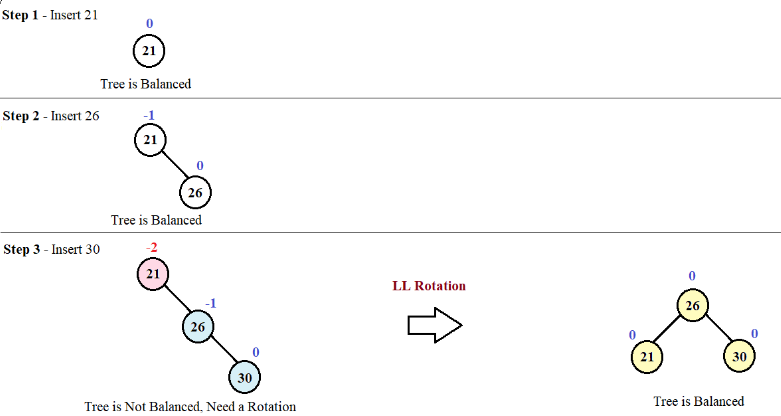
\includegraphics[width=.85\textwidth]{AVL1.png}
          \end{figure}

          \begin{figure}[H]
              \centering
              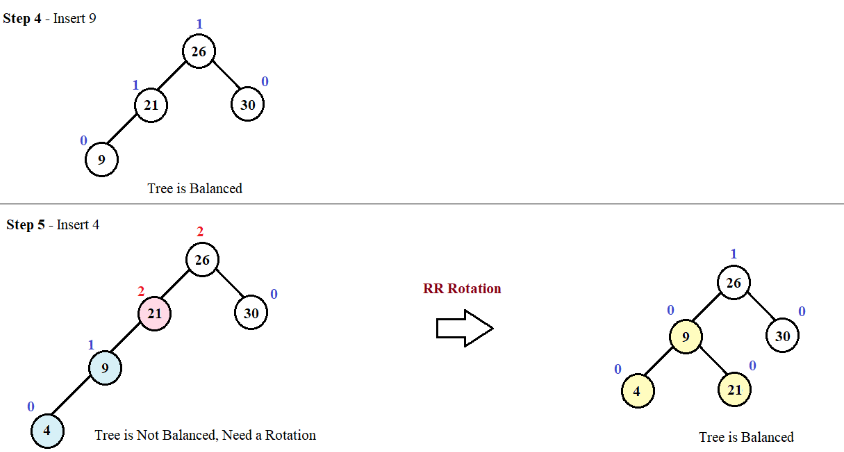
\includegraphics[width=.85\textwidth]{AVL 2.png}
          \end{figure}

          \begin{figure}[H]
              \centering
              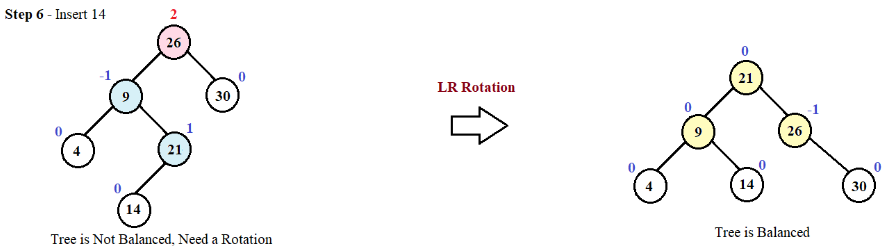
\includegraphics[width=.85\textwidth]{AVL 3.png}
          \end{figure}
    \item \textbf{Compute the time complexity of AVL tree creation?}\\

          The time complexity of creating an AVL tree depends on the number of elements n that need to be inserted. In the worst case, when the elements are inserted in sorted order, the time complexity of AVL tree creation is O(n log n), since each insertion may require a series of rotations to maintain balance. In the best case, when the elements are inserted in a balanced manner, the time complexity of AVL tree creation is O(n). This is because each node is inserted and balanced in constant time, so the total time is proportional to the number of nodes inserted.

          In practice, AVL trees are very efficient for creating and maintaining a dictionary because they provide fast search, insertion, and deletion operations. However, they do require additional memory to store the balance factor of each node, and the overhead of maintaining balance can add to the running time of operations. Overall, AVL trees are a good choice for applications that require a balanced binary search tree and where the number of insertions and deletions is not too frequent.
\end{enumerate}
\end{document}